\section{Positive and Unlabeled Learning}
\label{sec:pulearning}

\textit{One sentence summary of Positive and Unlabeled Learning}

%%%%%%%% TEXT PU Learning setup

\paragraph{Formulation}
\noindent
\textit{This part should explain the Positive and Unlabeled Learning setup with mathematical representation when necessary.}


%%%%%%%% TEXT Modeling
\paragraph{Weighted Logistic Regression}
\noindent
\textit{This part should discuss the linear model for observing positive conditioning on true positive and its relationship to changing the class weight.}


%%%%%%%% TEXT Exponential loss
\paragraph{Exponential Loss for unlabeled examples}
\noindent
\textit{This part should explain why the exponential loss could perform better than the cross-entropy loss, potentially with a figure of 2D Gaussians.}


%%%%%%%% TEXT Expontial loss FADE IN
\noindent
\textit{This paragraph should explain why fade-in was introduced to avoid all-positive inital prediction}


%%%%%%%% TEXT Imbalanced
\noindent
\textit{This part should explain the influence of the imbalanced problem and how to overcome.}



%%%%%%%% FIGURE MOONS
\begin{figure*}
\begin{center}
% \fbox{\rule{0pt}{2in} \rule{.9\linewidth}{0pt}}
   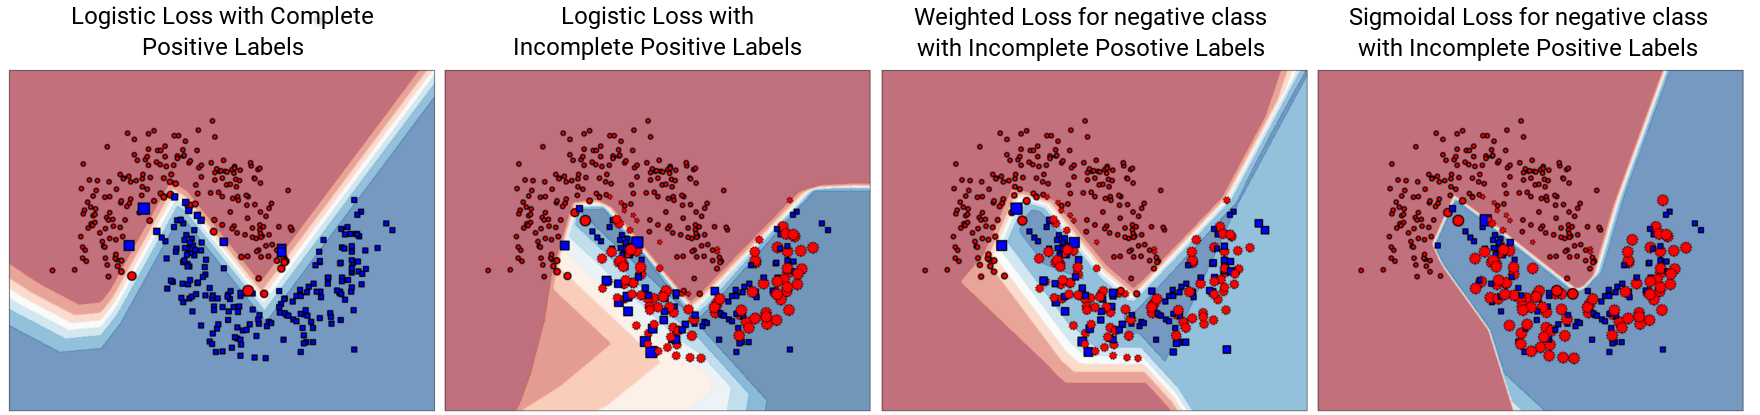
\includegraphics[width=0.95\linewidth]{img/moons.png}
\end{center}
   \caption{2D moons dataset with non-linear separable decision boudary. Four hundreds samples per class were drawn randomly from two interleaving half circles with noises added with a minor standard deviation. A \textbf{red circle} indicates an example labelled as positive whilst a \textbf{blue square} indicates the example has a negative label. The \textbf{leftmost} figures have complete positive labels, meaning the positive and negative labels are all correct, whereas, in \textbf{the other figures} only half of the positives were correctly labelled and the rest were mixed with the negative samples. The \textbf{background colors} represent the probability for the area to be positive given by the classifier trained with the given samples and labels: \textbf{red} for high probability areas, \textbf{blue} for low probability areas and \textbf{white} for the class transition areas, i.e.decision boundaries. The \textbf{size of the markers} in the top row denotes the per-class normalized training losses and the \textbf{size of the markers} in the bottom row the per-class normalized derivatives w.r.t the output of the last layer for the trained Multilayer Perceptron (MLP) with the different losses.}
\label{fig:moons}
\end{figure*}


%%%%%%%% FIGURE Losses
\begin{figure}[t]
\centering
% \fbox{\rule{0pt}{2in} \rule{0.9\linewidth}{0pt}}
   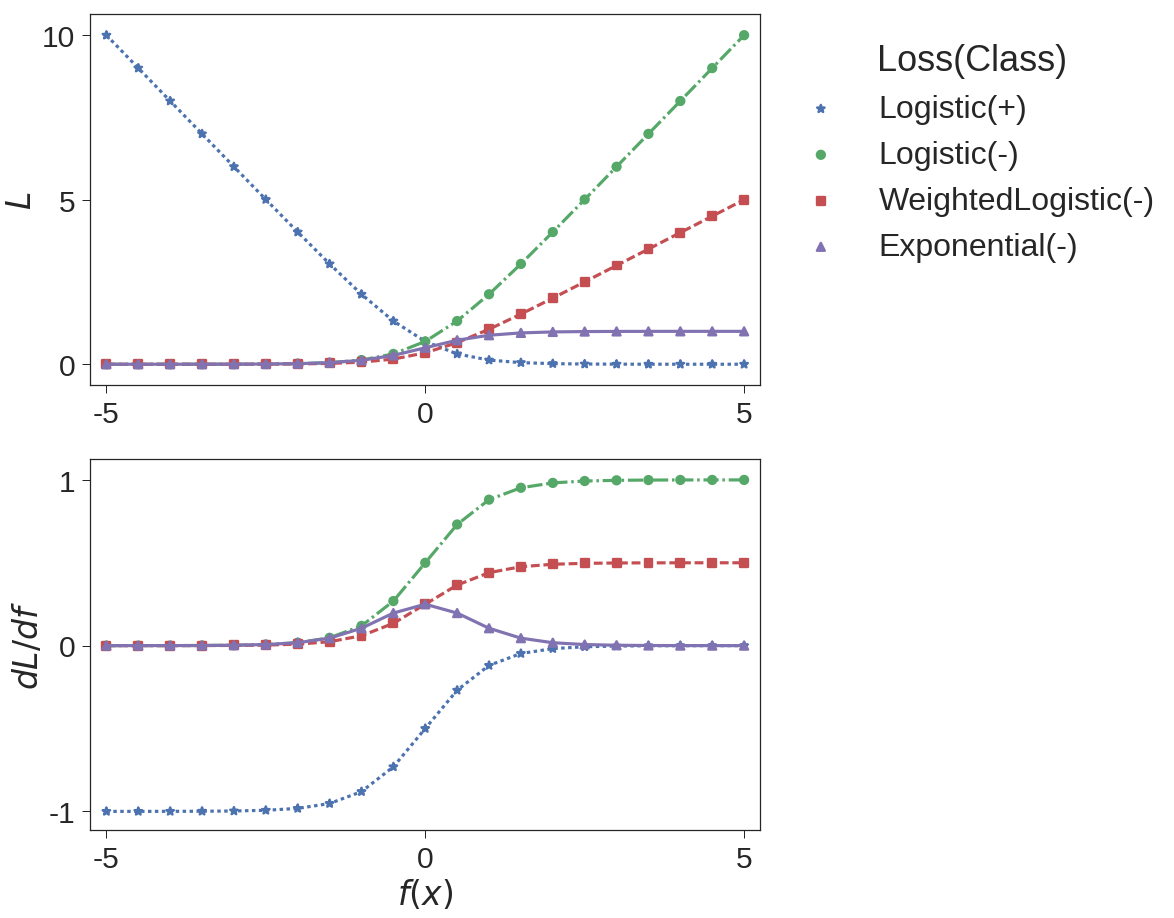
\includegraphics[width=0.95\linewidth]{img/losses.png}
\caption{The Logistic Loss, Weighted Logistic Loss, Exponential Loss and their dirivatives with respect to the model output.}
\label{fig:losses}
\end{figure}


%%%%%%%% FIGURE Varying positive annotating percetage
\begin{figure}[t]
\centering
\fbox{\rule{0pt}{2in} \rule{0.9\linewidth}{0pt}}
  %  \includegraphics[width=0.95\linewidth]{img/}
\caption{Varying percentage of annotated positives 10\%, 20\%, 50\%, 80\% and 100\% with images from CIFAR10 as the positives and images from CIFAR110 as the negatives.}
\label{fig:pct_annotating}
\end{figure}

%%%%%%%% TABLE CIFAR10
\begin{table}[t]
\resizebox{\columnwidth}{!}{
\centering
\begin{tabular}{ll|llll}
Annotation  & Loss & acc. & prec. & rec. & $F_1$ \\
\hline
Complete    & CrossEntropyU    & 0.87 & 0.88 & 0.82 & 0.85 \\
50\%(P+N)   & CrossEntropyU    & 0.83 & 0.84 & 0.78 & 0.80 \\
50\%P+U     & CrossEntropyU    & 0.61 & 0.92 & 0.30 & 0.38 \\
50\%P+U     & WeightedU        & 0.66 & 0.93 & 0.39 & 0.51 \\
50\%P+U     & ExponentialU     & 0.82 & 0.86 & 0.73 & 0.78 \\
50\%P+U     & BootstrapHard    & 0.74 & 0.81 & 0.60 & 0.67 \\
50\%P+U     & DropoutRegularization & & & & \\
\end{tabular}
}
\caption{Image classification with positive examples partially annotated. The complete dataset contains images from CIFAR10 as the \textbf{positive} (P) set and images from CIFAR110 as the \textbf{negative} (N) set. The unannotated positive examples from P set construct the \textbf{unlabeled} (U) set together with the N set.}
\end{table}


%%%%%%%% TABLE
\begin{table}[t]
\resizebox{\columnwidth}{!}{
\centering
\begin{tabular}{ll|llll}
Annotation  & Loss & pixel acc. & mean acc. & mean IU & f.w. IU \\
\hline
Complete    & CrossEntU    &  &  & & \\
50\%(P+N)   & CrossEntU    & & & & \\
50\%P+U     & CrossEntU    & & & & \\
50\%P+U     & WeightedU        &  &  & & \\
50\%P+U     & ExponentialU     &  &  & & \\
50\%P+U     & BootstrapHard    &  &  & & \\
50\%P+U     & DropoutReg & & & & \\
\end{tabular}
}
\caption{Image semantic segmentation with images contain single instance only from the PASCAL VOC2011 segmentation dataset. The complete \textbf{positive} (P) set denotes the foreground instances and the \textbf{negative} (N) set consists of the background. The unannotated instances from P set construct the \textbf{unlabeled} (U) set together with the N set.}
\end{table}
